\lstset{language=bash}
\chapter{OpenXENManager}
\section{Présentation}
XenseMaking Project développe un client lourd, ainsi qu'un client
web, pour manager XenServer. C'est un clone du XenCenter, qui fonctionne
avec Linux, BSD, Windows et MacOSX, alors que le XenCenter ne fonctionne
qu'avec Windows. OpenXenManager/OpenXenCenter un le client lourd qui
permet de manager XenServer.Il a été développé en Python avec pygtk
et gtk-vnc.
Les fonctionnalités actuellement implémentées sont les suivantes :
\begin{itemize}
\item monitoring des machines virtuelles - accès à la console des machines virtuelles
\item opérations d'administration (démarrage, arrèt, reboot, ...)
\item création de machines virtuelles
\end{itemize}
\section{Installation}
Pour l'installation nous avons besoin des paquets suivant:
\begin{lstlisting}
apt-get install subversion bzip2 python-glade2 python-gtk-vnc shared-mime-info graphviz
\end{lstlisting}
On télécharge la dernière version d'openxenmanager dans le dépot subversion
\begin{lstlisting}
svn co https://openxenmanager.svn.sourceforge.net/svnroot/openxenmanager openxenmanager
\end{lstlisting}
On se déplace dans le répertoire trunk:
\begin{lstlisting}
cd openxenmanager/trunk
\end{lstlisting}
Finalement on lance openxenmanager avec la commande suivante
\begin{lstlisting}
python window.py
\end{lstlisting}
Une interface graphique d'openxenmanger apparait.
\section{Utilisation}
Pour l'instant nous n'avons toujours pas réussi à utiliser ce logiciel. DU a diverses difficultées (pas de service distant sous squeeze et plus de xen lors de la migration sous unstable).
\chapter{Xen Cloud Platform}
\section{installation}
\begin{figure}
\begin{center}
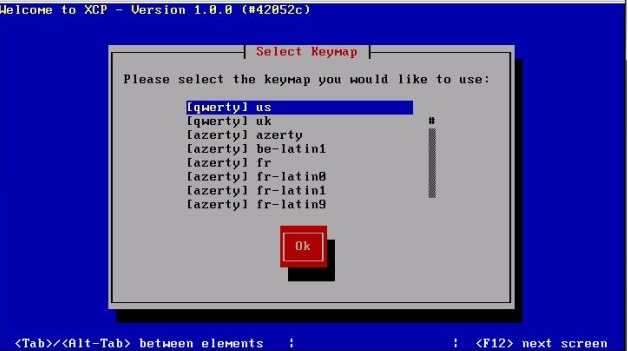
\includegraphics[width=350pt]{images/1.png}
\end{center}
\caption{On choisit le  type de clavier}
\end{figure}
\begin{figure}
\begin{center}
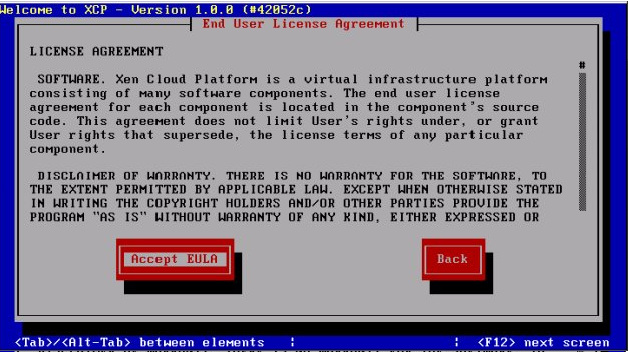
\includegraphics[width=350pt]{images/2.png}
\end{center}
\caption{On accepte la licence}
\end{figure}
\begin{figure}
\begin{center}
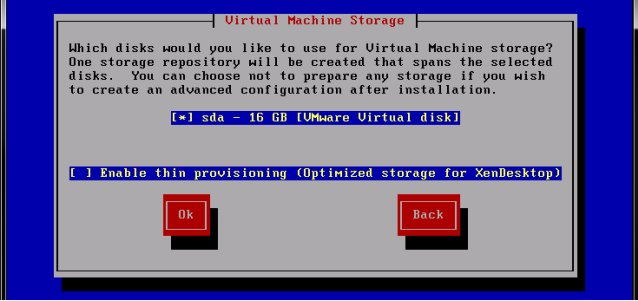
\includegraphics[width=350pt]{images/3.png}
\end{center}
\caption{Choix du disque d'installation}
\end{figure}
\begin{figure}
\begin{center}
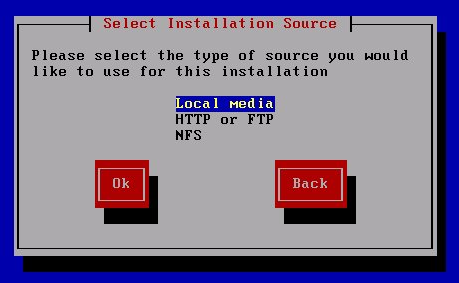
\includegraphics[width=350pt]{images/4.png}
\end{center}
\caption{Choix de la source d'installation}
\end{figure}
\begin{figure}
\begin{center}
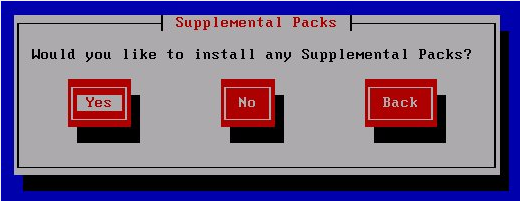
\includegraphics[width=350pt]{images/5.png}
\end{center}
\caption{Paquets additionnels}
\end{figure}
\begin{figure}
\begin{center}
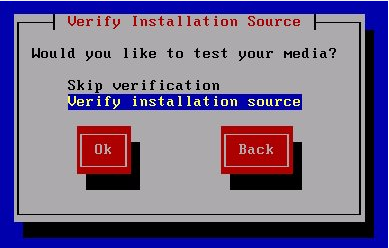
\includegraphics[width=350pt]{images/6.png}
\end{center}
\caption{Vérification de la source d'installation}
\end{figure}
\begin{figure}
\begin{center}
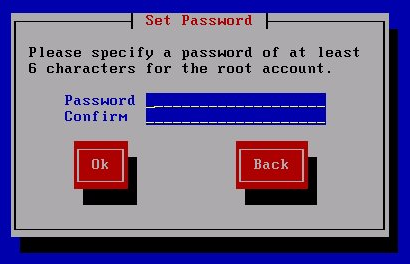
\includegraphics[width=350pt]{images/7.png}
\end{center}
\caption{Choix du password}
\end{figure}
\begin{figure}
\begin{center}
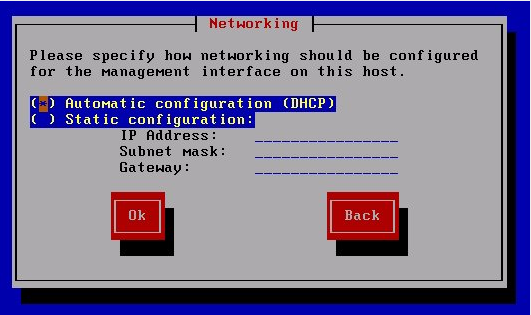
\includegraphics[width=350pt]{images/8.png}
\end{center}
\caption{Configuration du réseau}
\end{figure}
\begin{figure}
\begin{center}
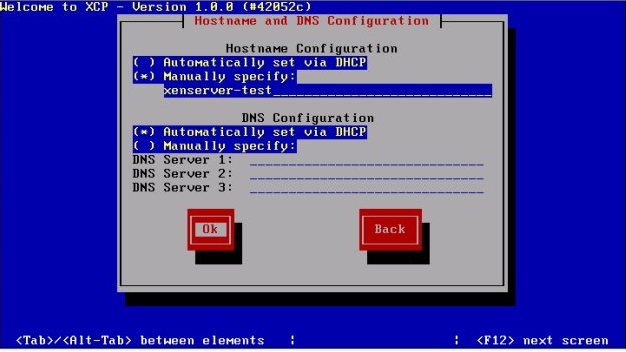
\includegraphics[width=350pt]{images/9.png}
\end{center}
\caption{Configuration du DNS}
\end{figure}
\begin{figure}
\begin{center}
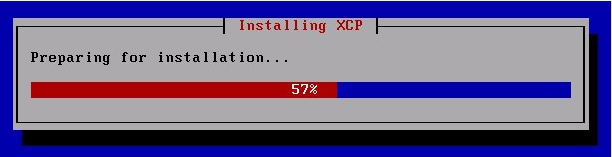
\includegraphics[width=350pt]{images/10.png}
\end{center}
\caption{Installation}
\end{figure}
\begin{figure}
\begin{center}
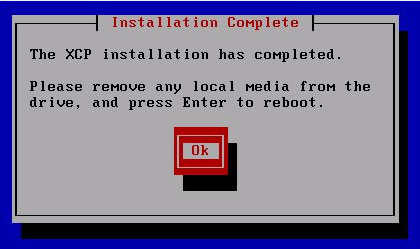
\includegraphics[width=350pt]{images/11.png}
\end{center}
\caption{Installation complète}
\end{figure}
